%\documentclass{jss}
\documentclass[article, nojss]{jss}
\usepackage[OT1]{fontenc}
\usepackage[utf8]{inputenc}
\usepackage{graphicx}
%symbole math de l'American Mathematical Society (AMS)
\usepackage{amsfonts,amssymb,amsmath,amsthm}


%\usepackage{cite}
\usepackage{draftwatermark}
\SetWatermarkText{Draft}
\SetWatermarkScale{1.5}

%\usepackage{myVignette}

%\VignetteIndexEntry{The MBBEFD package}
%\VignetteKeywords{vig1}
%\VignettePackage{mbbefd}
% need no \usepackage{Sweave.sty}

%\SweaveOpts{prefix.string=Figures/fig}
%%%%%%%%%%%%%%%%%%%%%%%%%%%%%%
%% declarations for jss.cls %%%%%%%%%%%%%%%%%%%%%%%%%%%%%%%%%%%%%%%%%%
%%%%%%%%%%%%%%%%%%%%%%%%%%%%%%

%% almost as usual
\author{Giorgio Alfredo Spedicato\\ Ph.D C.Stat ACAS \And Christophe Dutang\\ University of Le Mans city}
\title{The \pkg{mbbefd} Package: A Package for handling destruction rates in \proglang{R} including
MBBEFD distributions}

%% for pretty printing and a nice hypersummary also set:
\Plainauthor{Giorgio Alfredo Spedicato, Christophe Dutang} %% comma-separated
\Plaintitle{The mbbefd Package: A Package for handling MBBEFD exposure curves in R} %% without formatting
\Shorttitle{The mbbefd package} %% a short title (if necessary)
%% an abstract and keywords
\Abstract{The package models MBBEFD distribution providing density, quantile, distribution and random generation functions. In addition it provides exposure curves for the MBBEFD distribution family.
}
\Keywords{mbbefd, exposure curves, reinsurance, non-life insurance}
\Plainkeywords{mbbefd, exposure curves, reinsurance, non-life insurance} %% without formatting
%% at least one keyword must be supplied

%% publication information
%% NOTE: Typically, this can be left commented and will be filled out by the technical editor
%% \Volume{13}
%% \Issue{9}
%% \Month{September}
%% \Year{2004}
%% \Submitdate{2004-09-29}
%% \Acceptdate{2004-09-29}

%% The address of (at least) one author should be given
%% in the following format:
\Address{
  Giorgio Alfredo Spedicato, Ph.D C.Stat ACAS\\
  StatisticalAdvisor\\
  Paderno Dugnano\\
  20037 Italy\\
  E-mail: \email{spedicato\_giorgio@yahoo.it}\\
  URL: \url{www.statisticaladvisor.com}
}


%% for those who use Sweave please include the following line (with % symbols):
%% need no \usepackage{Sweave.sty}

%% end of declarations %%%%%%%%%%%%%%%%%%%%%%%%%%%%%%%%%%%%%%%%%%%%%%%

\newcommand{\ind}{1\!\!1}
%sets
\newcommand{\R}{\mathbb R}
\newcommand{\N}{\mathbb N}
\newcommand{\calD}{\mathcal D}

%system
\newcommand{\systL}{\left\{\begin{array}{ll}}
\newcommand{\systR}{\end{array}\right.}
\newcommand{\matL}{\left(\begin{matrix}}
\newcommand{\matR}{\end{matrix}\right)}
\newcommand{\detL}{\left|\begin{matrix}}
\newcommand{\detR}{\end{matrix}\right|}



\newcommand{\Sconcordance}[1]{%
  \ifx\pdfoutput\undefined%
  \csname newcount\endcsname\pdfoutput\fi%
  \ifcase\pdfoutput\special{#1}%
  \else%
   \begingroup%
     \pdfcompresslevel=0%
     \immediate\pdfobj stream{#1}%
     \pdfcatalog{/SweaveConcordance \the\pdflastobj\space 0 R}%
   \endgroup%
  \fi}
  
\begin{document}
\input{mbbefd-concordance}




\maketitle



%%%%%%%%%%%%%%%%%%%%%%%%%%%%%%%%%%%%%%%%%%%%%%%
\section{Introduction}

The \pkg{mbbefd} package provides function to use Maxwell-Bolzano, Bose-Einstein, Fermi-Dirac probability distributions, introduced by \cite{bernegger97}, within \proglang{R} statistical software \citep{rSoftware}.\\ Such kind of distributions are widely used in the pricing of non-life reinsurance contracts and yet they are not present in any R package.\\

The paper is structured as follows: Section~\ref{sec:review} discusses review the theory (mathematics and actuarial application) of MBBEFD distributions, Section~\ref{sec:package} shows the package's features, applied examples are shown in Section~\ref{sec:examples} while the issue of fitting MBBEFD curves to empirical data is discussed in Section~\ref{sec:fitting}.\\



%______________________________________________________
\section{Exposure curves}
We first present the exposure curve of a random variable.
The exposure curve naturally arises in the insurance context when considering $d$ as the normalized 
deductible and $X$ the normalized loss. 
That is respectively the ratio of the deductible value on the maximum possible loss
and the loss value on the maximum possible loss.
This quantity is even more appealing in the reinsurance context where the deductible is
the priority and the maximum possible loss is the sum of the priority and
the limit of the reinsurance treaty, see \cite{bernegger97} and \cite{mahler}.


%---
\subsection{Definition}
Let $X$ be a random variable valued in the unit interval $I=[0,1]$ with distribution function $F_X$.
The exposure curve function of $X$ is defined as the ratio of the limited expected value and the expectation
$$
G_X(d) = \frac{E(\min(X,d))}{E(X)}, 
$$
for $d\in [0,1]$.
Since $X$ is a positive random variable, we have
$$
G_X(d) = \frac{\int_0^d (1-F_X(x))dx }{\int_0^1 (1-F_X(x))dx }.
$$
Note that the exposure curve is a concave function for $d\in]0,1[$. 

There is a direct link between the distribution function and the exposure curve.
Since 
$$
F_X(x) = \left(1- \frac{G_X'(x)}{G_X'(0)}\right)\ind_{[0,1[}(x) + \ind_{[1,+\infty[}(x),
$$
defining the exposure curve or the distribution function is equivalent.
The exposure curve is also a concave increasing function, see e.g.~\cite{antal03}.

%---
\subsection{Examples}

\subsubsection{Uniform distribution}
\label{sec:unif}

The most trivial example of exposure curve is obtained for the uniform distribution on $I$.
We consider $F_X(x)=x$ leading to
$$
G_X(d) 
= d(2-d).
$$

%---
\subsubsection{Example: beta distribution}
\label{sec:beta}

A more interesting example is obtained for the Beta distribution on $I$ 
(e.g.~\cite{kotzjohnsonbalak94v2})
for which the density is $f_X(x) = x^{a-1}(1-x)^{b-1}/\beta(a,b)$ for $x\in ]0,1[$ and $a,b>0$
where $\beta(.,.)$ denotes the 
beta function, see e.g.~\cite{nist10}.
The distribution function is obtained in terms of the incomplete beta ratio function 
$F_X(x) = \beta(x;a,b)/\beta(a,b) = I(x;a,b)$.
We get
$$
G_X(d) %= \frac{1 - I(d;a,b) \frac{b}{a+b} - \frac{d^a(1-d)^b}{(a+b)\beta(a,b)} }{a/(a+b)}
= \frac{a+b}{a} - I(d;a,b) \frac{b}{a} - \frac{d^a(1-d)^b}{a\beta(a,b)},
$$
where $\beta(.;.,.)$ denotes the incomplete beta function.



%---
\subsection{Empirical exposure curve}
We recall that the empirical cumulative distribution of a sample $X_1,\dots, X_n$ is 
the following step function
$$
F_n(t) = \frac{1}{n} \sum_{i=1}^n \ind_{X_i\leq t}.
$$
Similarly, we define the empirical exposure curve function as
$$
G_n(t) = \frac{\frac{1}{n} \sum_{i=1}^n \min(X_i, t)}{\frac{1}{n} \sum_{i=1}^n X_i}.
$$

%---
\subsection{Use case}
The uniform and the beta distributions are already implemented in \proglang{R} 
with \code{d,p,q,runif} and  \code{d,p,q,rbeta} functions.
We add a new function computing the exposure curve as well as for the non-parametric version $G_n$.

\begin{Schunk}
\begin{Sinput}
R> library(mbbefd)
R> ecunif(0:4/4)
\end{Sinput}
\begin{Soutput}
[1] 0.0000 0.4375 0.7500 0.9375 1.0000
\end{Soutput}
\begin{Sinput}
R> ecbeta(0:4/4, 3, 2)
\end{Sinput}
\begin{Soutput}
[1] 0.0000000 0.4111328 0.7604167 0.9599609 1.0000000
\end{Soutput}
\begin{Sinput}
R> eecf(rbeta(100, 3, 2))
\end{Sinput}
\begin{Soutput}
Empirical Exposure Curve Function 
Call: eecf(rbeta(100, 3, 2))
 x[1:100] = 0.16479, 0.19761, 0.20338,  ..., 0.94344, 0.96718
\end{Soutput}
\end{Schunk}



%______________________________________________________
\section{One-inflated distributions}\label{sec:oidistr:generic}

%---
\subsection{Characterizations}\label{sec:oidistr:generic:charac}
Let us consider a continuous distribution function $F_0$ of a random variable $X_0$. 
The corresponding distribution function of the one-inflated random variable $X_1$ is 
$$
F_1(x) = (1-p_1) F_0(x) + p_1 \ind_{[1,+\infty[}(x).
$$
There is no density but an improper density $(1-p)F_0'(x)$ and a probability mass $p_1$ at $x=1$.


%---
\subsection{The one-inflated beta distribution}
We consider the one-inflated beta distribution.
Using Section \ref{sec:beta}, we obtain the following distribution function
$$
F_X(x) = 
\systL
0 & \text{if } x<0 \\
I(x;a,b)(1-p_1) & \text{if } 0\leq x <1 \\
1 & \text{if } x\geq 1
\systR
$$
where $I(x;a,b)$ denotes the incomplete beta ratio function.
This leads to a non-null probability at $x=1$, $P(X=1)=p_1$.
The improper density function is 
$$
\tilde f_X(x) = (1-p_1) \frac{x^{a-1}(1-x)^{b-1}}{\beta(a,b)}.
$$
The expectation is
$$
E(X) 
= p_1 + (1-p_1)\frac{a}{a+b}.
$$
The exposure curve is 
$$
G_X(d) =  
\frac{(1-p_1) \left(1 - I(d;a,b) \frac{b}{a+b} - \frac{d^a(1-d)^b}{(a+b)\beta(a,b)}\right) + p_1d
}{p_1 + (1-p_1)\frac{a}{a+b}}.
$$


%---
\subsection{Use case}
Classical one-inflated distributions are implemented in the package:
\begin{Schunk}
\begin{Sinput}
R> doibeta(0:4/4, 3, 2, 1/2)
\end{Sinput}
\begin{Soutput}
[1] 0.00000 0.28125 0.75000 0.84375 0.50000
\end{Soutput}
\begin{Sinput}
R> poibeta(0:4/4, 3, 2, 1/2)
\end{Sinput}
\begin{Soutput}
[1] 0.00000000 0.02539063 0.15625000 0.36914062 1.00000000
\end{Soutput}
\end{Schunk}



%______________________________________________________
\section{The MBBEFD distribution, first parametrization}

We denote this first parametrization by $MBBEFD(a,b)$.
We define the parameter domain $\calD_{a,b}$ as 
\begin{equation}
\calD_{a,b} = \{(a,b)\in\R^2, a+1>0, a(1-b)>0, b>0\}
\cup \{(a,b), a=+\infty, b<1\}.
\label{eq:paramdomain:mbbefd:ab}
\end{equation}
Let us note that this domain includes two particular sets $\calD_{a,1}=\{(a,1), a+1>0\}$ and $\calD_{0,b}=\{(0,b), b>0\}$.

%---
\subsection{Characterization by the exposure curve}
The MBBEFD distribution is defined by the following exposure curve for $(a,b)\in\calD_{a,b}$
\begin{equation}
\forall x\in I,~
G_X(x) = 
\systL
\frac{\ln(\frac{a+b^x}{a+1})}{\ln(\frac{a+b}{a+1})} & \text{if } a(1-b) >0 \\
\frac{1-b^x}{1-b} & \text{if } a=+\infty \text{ and } b<1 \\
x & \text{if } a=0 \text{ or } b=1. \\
\systR
\label{expcurve:mbbefd:ab}
\end{equation}
The two special cases of $a(1-b)=0$ 
correspond to $\calD_{a,1}$ and $\calD_{0,b}$.
Note that the denominator is a normalizing constant to ensure the term belongs to $[0,1]$.



%---
\subsection{Distribution, density and quantile functions}
Differentiating $G_X$, we obtain the following distribution function
 for $(a,b)\in\calD_{a,b}$
\begin{equation}
\forall x\in I,~
F_X(x) = 
\systL
\left(1-\frac{(a+1)b^x}{a+b^x}\right)\ind_{[0,1[}(x) + \ind_{[1,+\infty[}(x) & \text{if } a(1-b) >0 \\
(1-b^x)\ind_{[0,1[}(x) + \ind_{[1,+\infty[}(x) & \text{if } a=+\infty \text{ and } b<1 \\
\ind_{[1,+\infty[}(x) & \text{if } a=0 \text{ or } b=1. \\
\systR
\label{cdf:mbbefd:ab}
\end{equation}
Note that the MBBEFD distribution is a mixed-type distribution with mass probability at $x=1$
\begin{equation}
P(X=1)  = \frac{(a+1)b}{a+b} = p_{a,b},
\label{mass0:mbbefd:ab}
\end{equation}
which equals to 1 when $a(1-b)=0$. In other words, for $\calD_{a,1}$ and $\calD_{0,b}$, $X$ has a Dirac distribution at $x=1$.
When $a=+\infty$, the total loss probability is $P(X=1)=b$.

For $a(1-b)>0$, the improper density function is 
\begin{equation}
\tilde f_X(x) 
\systL
-\frac{a(a+1)b^x\ln(b)}{(a+b^x)^2}\ind_{[0,1[}(x) & \text{if } a(1-b) >0 \\
-\ln(b)b^x\ind_{[0,1[}(x)  & \text{if } a=+\infty \text{ and } b<1 \\
0 & \text{if } a=0 \text{ or } b=1. \\
\systR
\label{impd:mbbefd:ab}
\end{equation}
The quantile function is 
\begin{equation}
\forall p\in [0,1],~
q_X(p) = 
\systL
\frac{\ln\left(\frac{(1-p)a}{a+p}\right)}{\ln(b)} \ind_{[0,1-p_{a,b}[}(p) + \ind_{[1-p_{a,b},1]}(p)  & \text{if } a(1-b) >0 \\
\frac{\ln(1-p)}{\ln(b)}\ind_{[0,1-b[}(p) + \ind_{[1-b,1]}(p)   & \text{if } a=+\infty \text{ and } b<1 \\
\ind_{]0,1]}(p) & \text{if } a=0 \text{ or } b=1. \\
\systR
\label{q:mbbefd:ab}
\end{equation}


%---
\subsection{Moments}
Using the definition of the exposure curve, we have
$E(X) = 1/G_X'(0).$
The expectation for $MBBEFD(a,b)$ is
$$
E(X)=\frac{\ln(\frac{a+b}{a+1})}{\ln(b)} (a+1).
$$
When $a=0$ or $b=1$, the expectation is simply $E(X)=1$.



%______________________________________________________
\section{The MBBEFD distribution, second parametrization}

%---
\subsection{Parameter domain}

For fitting purposes and for verifying parameter constraints, 
\cite{bernegger97} proposed a second parametrization $MBBEFD(g,b)$.
Using the following parameter $g=1/p_{a,b}$, it is possible to reformulate the $MBBEFD(a,b)$.
That is
$$
g= \frac{a+b}{(a+1)b}
\Leftrightarrow
a=\frac{(g-1)b}{1-gb}.
$$
So $g\geq 1$ guarantees that $\frac{a+b}{(a+1)b}\in [0,1]$, in addition to $b>0$.
The special case $g=1$ leading to a Dirac distribution at $x=1$ corresponds to $a(1-b)=0$ in the previous parametrization.
The parameter domain is
$$
\widetilde{\calD}_{g,b}= \left\{
(g,b)\in\R^2, b>0, g\geq 1
\right\}.
$$


%---
\subsection{Characterization by the exposure curve}

The exposure curve is defined for $x\in[0,1]$ as
\begin{equation}
G_X(x)=
\systL
\frac{\ln(\frac{(g-1)b}{1-b}+\frac{1-gb}{1-b}b^x)}{\ln(gb)} & \text{ if } g>1, b\neq 1, b\neq 1/g \\
\frac{\ln(1+(g-1)x)}{\ln( g)} & \text{ if } g>1, b= 1 \\
\frac{1-b^x}{1-b} & \text{ if } g>1, bg= 1 \\
x & \text{ if } g=1 \text{ or } b= 0
\systR
\label{expcurve:mbbefd:gb}
\end{equation}
Note that the case $g>1, bg=1$ implies $g=1/b, b<1$.


%---
\subsection{Distribution, density and quantile functions}

The resulting distribution function is
\begin{equation}
F_X(x)=
\systL
\left(1- \frac{1-b}{(g-1)b^{1-x}+1-gb}\right)\ind_{[0,1[}(x) + \ind_{[1,+\infty[}(x) & \text{ if } g>1, b\neq 1, b\neq 1/g \\
\left(1- \frac{1}{1+(g-1)x}\right)\ind_{[0,1[}(x) + \ind_{[1,+\infty[}(x) & \text{ if } g>1, b= 1 \\
(1-b^x)\ind_{[0,1[}(x) + \ind_{[1,+\infty[}(x) & \text{ if } g>1, bg= 1 \\
\ind_{[1,+\infty[}(x) & \text{ if } g=1 \text{ or } b= 0
\systR
\label{cdf:mbbefd:gb}
\end{equation}
As in the previous parametrization, there is a non-null probability at $x=1$, 
\begin{equation}
P(X=1)  = 1/g.
\label{mass0:mbbefd:gb}
\end{equation}
The improper density function is for $x\in ]0,1[$
\begin{equation}
\tilde f_X(x) = 
\systL
- \frac{(1-b)\ln(b)b^{1-x}}{((g-1)b^{1-x}+1-gb)^2}  & \text{ if } g>1, b\neq 1, b\neq 1/g \\
\frac{g-1}{(1+(g-1)x)^2} & \text{ if } g>1, b= 1 \\
-\ln(b) b^x  & \text{ if } g>1, bg= 1 \\
0 & \text{ if } g=1 \text{ or } b= 0
\systR
\label{impd:mbbefd:gb}
\end{equation}
The quantile function is 
\begin{equation}
\forall p\in [0,1],~
q_X(p) = 
\systL
\left(1-\frac{\ln\left(\frac{gb-1}{g-1} +\frac{1-b}{(1-p)(g-1)}\right)}{\ln(b)}  \right)
\ind_{[0,1-1/g[}(p) + \ind_{[1-1/g,1]}(p) & \text{ if } g>1, b\neq 1, b\neq 1/g \\
\frac{p}{(1-p)(g-1)}\ind_{[0,1-1/g[}(p) + \ind_{[1-1/g,1]}(p)  & \text{ if } g>1, b= 1 \\
\frac{\ln(1-p)}{\ln(b)}\ind_{[0,1-1/g[}(p) + \ind_{[1-1/g,1]}(p) & \text{ if }  g>1, bg= 1 \\
\ind_{]0,1]}(p) & \text{ if } g=1 \text{ or } b= 0
\systR
\label{q:mbbefd:gb}
\end{equation}


%---
\subsection{Moments}
Let us compute the first two moments.
$$
E(X) = 1/G_X'(0) = 
\systL
\frac{\ln(gb)(1-b)}{\ln(b)(1-gb)} & \text{ if } g>1, b\neq 1, b\neq 1/g \\
\frac{\ln(g)}{g-1}  & \text{ if } g>1, b= 1 \\
\frac{b-1}{\ln(b)} & \text{ if }  g>1, bg= 1 \\
1 & \text{ if } g=1 \text{ or } b= 0
\systR
$$


%______________________________________________________
\section{Examples of MBBEFD curves}\label{sec:examples}
The curve can be use to price property coverage and associate reinsurance treaties. Suppose a property expected loss to be 40K, MPL to be 2MLN. An XL coverage is available with a retention of 1Mln. The exposure curve that characterize the property is the usual one. Therefore the percentage of loss net and ceded is determined as it follows

\begin{Schunk}
\begin{Sinput}
R> net<-mbbefdExposure(x=1/2, a=0.2,b=0.04)*40000
R> ceded<-40000-net
\end{Sinput}
\end{Schunk}

and the expected loss as a percentage of total insured value is

\begin{Schunk}
\begin{Sinput}
R> expectedLoss<-1/dG(x=0,a=0.2,b=0.04)*40000
R> expectedLoss
\end{Sinput}
\begin{Soutput}
[1] 24000
\end{Soutput}
\end{Schunk}


Similarly, it is possible to draw the underluying suvival curve $S\left( x \right) = \frac{{G'\left( x \right)}}{{G'\left( 0 \right)}}$ using  Figure~\ref{fig:survival}.

\begin{figure}
\begin{center}
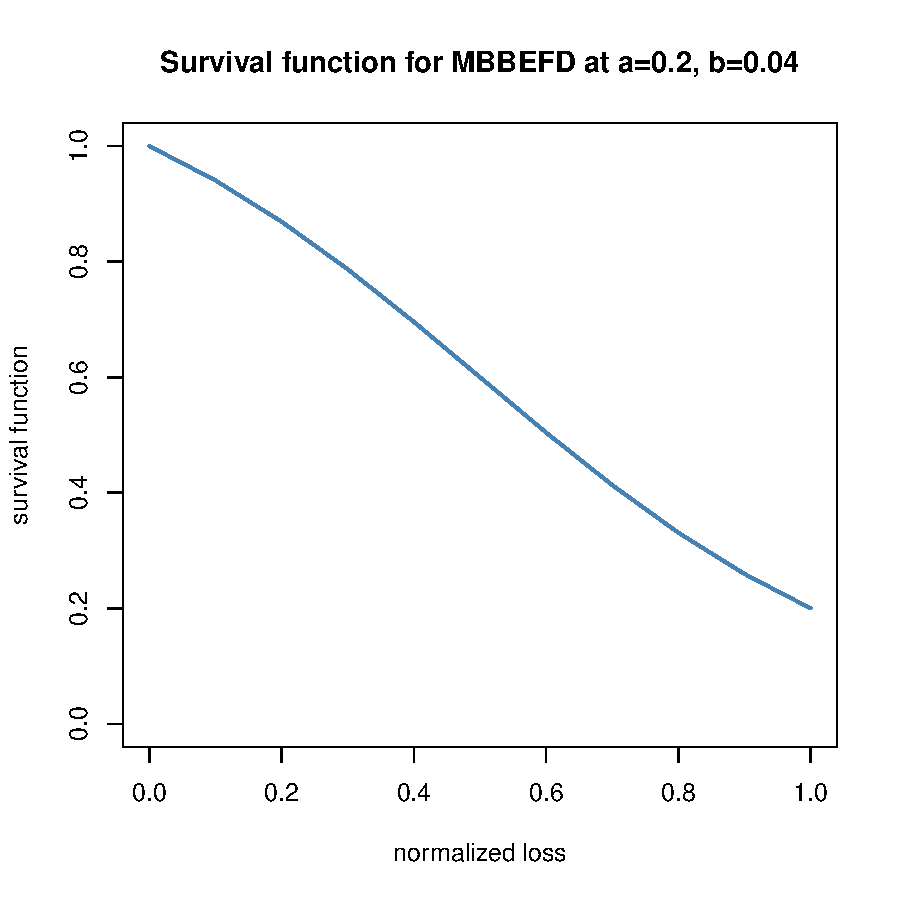
\includegraphics{mbbefd-survivalPlot}
\caption{Underlying survival curve}
\label{fig:survival}
\end{center}
\end{figure}


The probability of a maximum loss for such exposure curve is obtained evaluating the survival function at 1

\begin{Schunk}
\begin{Sinput}
R> pTotalLoss<-1-pmbbefd(q=1,a=0.2,b=0.04)
R> pTotalLoss
\end{Sinput}
\begin{Soutput}
[1] 0.2
\end{Soutput}
\end{Schunk}

Similarly, it is possible to assess the mean of the distribution underlying the exposure curve 


Quantile functions, distribution functions and density functions are defined as well. For example, the 60th percentile of the distribution above defined (i.e., how bad can be in 60\% of cases in terms of destruction rate) is

\begin{Schunk}
\begin{Sinput}
R> qmbbefd(p=0.6,a=0.2,b=0.04)
\end{Sinput}
\begin{Soutput}
[1] 0.7153383
\end{Soutput}
\end{Schunk}

whilst a loss worse than 80\% of IV could happen in 

\begin{Schunk}
\begin{Sinput}
R> 100*(1-pmbbefd(q=0.8,a=0.2,b=0.04))
\end{Sinput}
\begin{Soutput}
[1] 33.0895
\end{Soutput}
\end{Schunk}

cases out of 100.

It would be possible to simulate variates from the MBBEFD distribution using the 
random generation command \code{rmbbefd}.

\begin{Schunk}
\begin{Sinput}
R> simulatedLosses<-rmbbefd(n=10000,a=0.2,b=0.04)
R> mean(simulatedLosses)
\end{Sinput}
\begin{Soutput}
[1] 0.5979536
\end{Soutput}
\begin{Sinput}
R> sum(simulatedLosses==1)/length(simulatedLosses)
\end{Sinput}
\begin{Soutput}
[1] 0.1947
\end{Soutput}
\end{Schunk}

\begin{figure}
\begin{center}
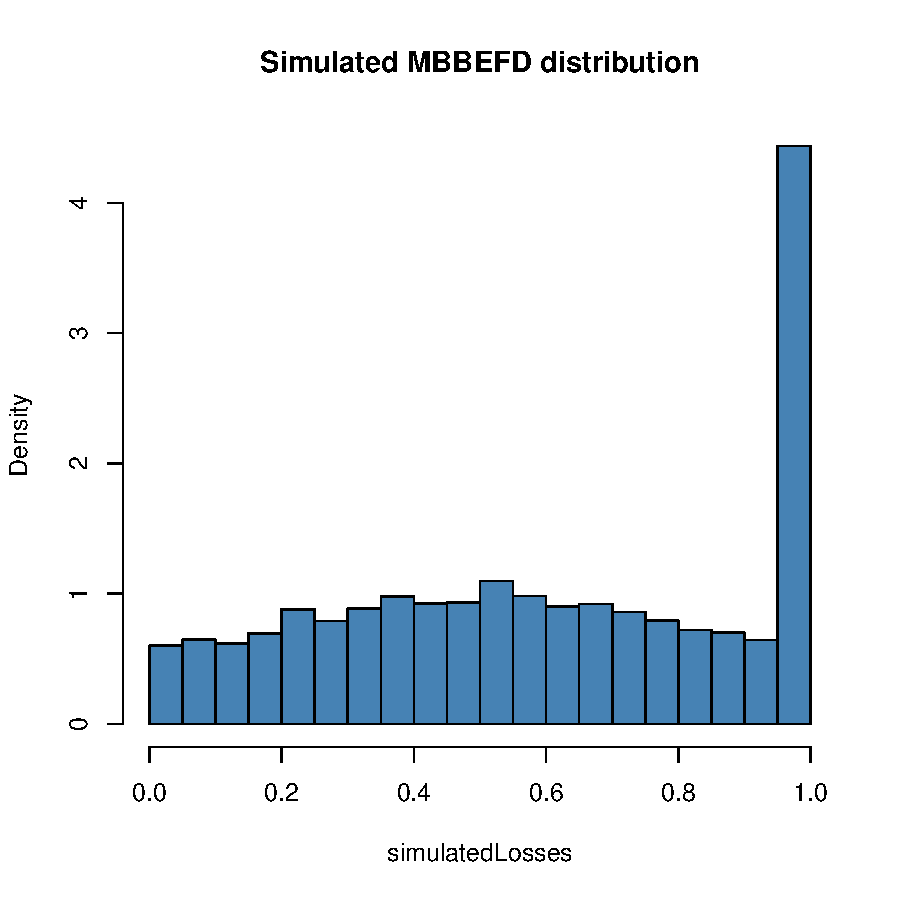
\includegraphics{mbbefd-distrPlot}
\caption{Exposure curve example}
\label{fig:G1}
\end{center}
\end{figure}




Finally another way to show the probability of total loss to be greater than zero is to show that the (numerical) integral between 0 and 1 of the density function is lower than 1, that is $1-F\left(1^- \right)$.

\begin{Schunk}
\begin{Sinput}
R> integrate(dmbbefd,lower=0, upper=1, a=0.2, b=0.04)
\end{Sinput}
\begin{Soutput}
0.8 with absolute error < 2.4e-13
\end{Soutput}
\end{Schunk}


\section{Fitting MBBEFD curves}\label{sec:fitting}


\cite{bernegger97} suggests an iterative process, based on the method of moments, in order to estimate the parameter of the 
distribution function, starting from known values of $p=\frac{1}{g}$ The algoritm outilined is:

\begin{enumerate}
  \item  Try $p_0 = m_2$, being $m_2$ the second empirical moment. Obtain $g_0=\frac{1}{p_0}$.
  \item  Solve for $b_0$ the equation $E\left[ x \right] = m_0 =  \frac{{\ln \left( {g_0*b_0} \right)}}{b_0}\frac{{1 - b_0}}{{1 - g_0*b}}$.
  \item Get the second theoretical moment, $E\left[ x^2 \right]$ of $x$ from estimated $b_0$ and $g_0$.
  \item Compare $E\left[ x^2 \right]$ to the empirical moment. Repeat the process modifying $p$ until the theoretical second moment is close to the empirical one enough (the second moment is an increasing function of p).
\end{enumerate}

Fitting a MBBEFD distribution is not easy. The result is sensible to initial values and appears to be instable.  We have applied the first three steps of this process in order to obtain initial estimates of $a$ and $b$ to feed the Maximum Likelihood estimation process using \pkg{fitdistrplus} package, \cite{fitdistrplusR}. We show two example one using both artificial data or real one (from package \pkg{copula}, \cite{copulaR}).


\begin{Schunk}
\begin{Sinput}
R> #get data
R> data1<-rmbbefd(n=1000,a = .2,b=.04)
R> data(loss, package = "copula")
R> data2<-pmin(1,pmax(0,loss$loss/loss$limit)) #capping loss data to lim
R> #functions used to initialize the parameters
R> #using one iteration of Method of Moments
R> 
R> #method of moments
R> 
R> giveFunction2Minimize<-function(mu,g) {
+    out = function(b) (mu - (log(g*b)*(1 - b))/( log(b)*(1 - g*b)) )^2
+    return(out)
+  }
R> giveFunction2Integrate<-function(b,g) {
+    out = function(x) x^2*dmbbefd(x,b=b,g=g)
+    return(out)
+  }
R> giveInits<-function(x) {
+    m0<-mean(x)
+    m2<-mean(x^2)
+    
+    #p<=1/g
+    
+    p0=m2 #m2 upper limit of p0
+    g=1/p0
+    
+    #equate 1rst moment to get the mean
+    myMin<-giveFunction2Minimize(mu=m0,g=g)
+    b<-nlm(f=myMin,p=.1)$estimate
+    
+    #return a
+    a=(g-1)*b/(1-g*b)
+    out<-list(a=a, b=b)
+    return(out)
+  }
R> ###fitting process
R> 
R> library(fitdistrplus)
R> #using close starting points
R> est1<-fitdist(data=data1,distr = "mbbefd",method = "mle",start=list(a=.9,b=.14))
R> est1
\end{Sinput}
\begin{Soutput}
Fitting of the distribution ' mbbefd ' by maximum likelihood 
Parameters:
    estimate Std. Error
a 0.18582390 0.02784803
b 0.03784101 0.00598667
\end{Soutput}
\begin{Sinput}
R> #using estimated starting points
R> inits2<-giveInits(x=data2)
R> est2<-fitdist(data=data2,distr = "mbbefd",method = "mle",start=inits2)
R> est1
\end{Sinput}
\begin{Soutput}
Fitting of the distribution ' mbbefd ' by maximum likelihood 
Parameters:
    estimate Std. Error
a 0.18582390 0.02784803
b 0.03784101 0.00598667
\end{Soutput}
\end{Schunk}



%\bibliographystyle{jss}
\bibliography{mbbefd}

\end{document}
